\def\student{Fabio Aubele \& Joshua Hörmann}

\def\bildbreite{.75\textwidth}

\documentclass[11pt,a4paper,oneside,english,listof=numbered,listof=leveldown,bibliography=totocnumbered]{scrartcl}

\usepackage[utf8]{inputenc}   % InputZeichenCodierung, zur RechtschreibKontrolle 
\usepackage[T1]{fontenc}       % [Europa]OutputZeichen, zur Silbentrennung
\usepackage{fontspec}
\setmainfont{Arial}

% erfordert texlive-fonts-recommended
\usepackage[german]{babel}    % SprachAnpassung, zur SilbenTrennung
\selectlanguage{german}

\usepackage[left=2.50cm, right=2.50cm, top=2.50cm, bottom=2.50cm]{geometry} % Seitenrand, die option showframe zeigt Rahmen um die einzelnen Bereiche der Seite an, damit die Abstände besser eingestellt werden können.

\usepackage{afterpage}         % auf neuer Seite plazieren
\usepackage[absolute]{textpos} % Textboxen an absolute Position setzen
\usepackage{setspace}          % Zeilenabstand anpassen (für Deckblatt)

\usepackage{graphicx}          % Bilder und Graphik
\usepackage{color}             % Farbige Schrift
\usepackage[dvipsnames]{xcolor}
\usepackage{longtable}         % Mehrseitige Tabelle
\usepackage{float}             % Positionieren der Bilder mit "H"

\usepackage[right]{eurosym}   % Darstellen von EURO Zeichenbiblatex
\usepackage[autostyle=true]{csquotes}

\usepackage[colorlinks,linkcolor=black, citecolor=gray, filecolor=black, urlcolor=blue]{hyperref}
\usepackage[style=numeric,backend=bibtex,sorting=none,natbib=true]{biblatex} 

\usepackage{listings}
\usepackage{color}
\renewcommand{\lstlistingname}{Code}
\usepackage{xcolor}

\definecolor{mygreen}{rgb}{0,0.4,0}
\definecolor{myred}{rgb}{0.8,0.16,0}
\definecolor{myrandom}{RGB}{255, 248, 246}
\definecolor{darkblue}{rgb}{0.0,0.0,0.6}
\lstset{
	belowcaptionskip=1\baselineskip,
	captionpos=b,
	lineskip=4pt,
	frame=L,
	xleftmargin=.037\textwidth, 
	xrightmargin=0pt,
	aboveskip=10pt,
	belowskip=-10pt,
	language=Python,
	showstringspaces=false,
	basicstyle=\footnotesize\ttfamily,
	keywordstyle=\color{darkblue},
	commentstyle=\itshape\color{mygreen},
	identifierstyle=\color{black},
	backgroundcolor=\color{myrandom}, 
	stringstyle=\color{myred},	
	numbers=left,
	numbersep=7pt,
}
\lstdefinelanguage{json}{
	belowcaptionskip=1\baselineskip,
	captionpos=b,
	lineskip=4pt,
	frame=L,
	xleftmargin=.037\textwidth, 
	xrightmargin=0pt,
	aboveskip=10pt,
	belowskip=-10pt,
	showstringspaces=false,
	basicstyle=\footnotesize\ttfamily,
	keywordstyle=\color{darkblue},
	commentstyle=\itshape\color{mygreen},
	identifierstyle=\color{black},
	backgroundcolor=\color{myrandom}, 
	stringstyle=\color{darkblue},	
	numbers=left,
	numbersep=7pt,
}

\usepackage{subcaption}
\usepackage[titletoc,title]{appendix}
\usepackage{pdfpages}
\usepackage{acronym}
\usepackage{enumitem}

\addbibresource{literature}

\usepackage{fancyhdr}          % Kopf und Fußzeile
\usepackage{lastpage}          % Gesamtanzahl der Seiten

\pagestyle{fancy}
\fancypagestyle{style1}{
\fancyhf{}
\renewcommand{\sectionmark}[1]{
	\markboth{\ifnum\value{section}=0 \else\thesection.\ \fi ##1}{}%
}
\fancyhead[L]{\nouppercase{\leftmark}}
\fancyhead[C]{}
\fancyhead[R]{\student}
\renewcommand{\headrulewidth}{0.4pt} %obere Trennlinie

\fancyfoot[L]{}
\fancyfoot[R]{Seite \thepage\ von \pageref{LastPage}}
}

\fancypagestyle{style2}{
	\fancyhf{}
	\renewcommand{\sectionmark}[1]{
		\markboth{\ifnum\value{section}=0 \else\thesection.\ \fi ##1}{}%
	}
	\fancyhead[L]{Abkürzungsverzeichnis}
	\fancyhead[C]{}
	\fancyhead[R]{\student}
	\renewcommand{\headrulewidth}{0.4pt} %obere Trennlinie
	
	\fancyfoot[L]{}
	\fancyfoot[R]{Seite \thepage\ von \pageref{LastPage}}
}

% Durchgehende Nummerierung von footnotes
\usepackage{remreset}
\makeatletter
\@removefromreset{footnote}{chapter}
\makeatother

\setlength{\parindent}{0pt}
\setlength{\parskip}{1.0em}
\renewcommand{\baselinestretch}{1.00}

\RedeclareSectionCommand[beforeskip=0.5em,afterskip=0.02em]{subparagraph}
\RedeclareSectionCommand[beforeskip=1.0em,afterskip=0.02em]{paragraph}

\begin{document}
	\pagestyle{style1}
	%%% Deckblatt - Hochschule Augsburg

\thispagestyle{empty}\null

%%% Logo - Hochschule Augsburg - Informatik
\begin{textblock}{10}(7.3,1.4)
	\begin{figure}[h]
		\centering
		
\includegraphics[width=0.55\textwidth]{figures/hsa_logo.pdf}
	\end{figure}
\end{textblock}

%%% Text unter Logo
\begin{textblock}{15}(11.8,2,9)
	\Large
	\textsf
	{
		\textbf
		{
			\textcolor[rgb]{1,0.4,0}
			{\\
			\begin{flushleft}
				Fakultät für\\
				Informatik
			\end{flushleft}
			}
		}
	}
\end{textblock}

%%% Infos Student
\begin{textblock}{20}(12,8,0)
	\begin{flushleft}
		\noindent
		\footnotesize
		\textsf
		{	
			\textbf
			{\\
				Verfasser der Arbeit:\\
				\vspace{6pt}
				Fabio Aubele\\
				Matrikelnummer: 955257\\
				Pfarrstraße 14a\\
				82140 Olching\\
				Telefon: +49 171 7900699\\
				fabioaubele95@hotmail.de\\
				\vspace{6pt}
				Joshua Hörmann\\				
				Matrikelnummer: 955524\\
				Anzengruberstr. 9\\
				82140 Olching\\
				Telefon: +49 151 46160769\\
				joshua.hoermann@feike-allgaeu.de\\
			}
		}
	\end{flushleft}
\end{textblock}

%%% Infos der Hochschule
\begin{textblock}{20}(12,11,15)
	\begin{flushleft}
		\noindent
		\footnotesize
			\textsf
			{
				\textcolor[rgb]{1,0,0.25}
				{\\
					Hochschule für angewandte\\
					Wissenschaft Augsburg\\
					University of Applied Sciences\\
					\vspace{6pt}
					An der Hochschule 1\\
					D-86161 Augsburg\\
					\vspace{6pt}
					Telefon +49 821 55 86-0\\
					Fax +49 821 55 86-3222\\
					www.hs-augsburg.de\\
					info@hs-augsburg.de\\
				}
			}	
			\textsf
			{
				\textbf
				{\\
					Fakultät für Informatik\\
					Telefon: +49 821 5586-3450\\
					Fax: \hspace{12.5pt} +49 821 5586-3449\\
				}			
			}	
	\end{flushleft}
\end{textblock}


%%% Textbox links - Informationen
\begin{textblock}{15}(1.55,2,5)
	\begin{flushleft}
		\begin{spacing} {1.2}
			\LARGE
				\textbf{Studienrichtung\\}
				\vspace{-5pt}
				\textbf{Informatik Master\\}
			\Huge
				\vspace{100pt}	
				\textcolor[rgb]{1,0.4,0}
				{\\
					\textbf{ArtBot - Dokumentation\\}
				}
				\vspace{-15pt}
			\Huge
				\textcolor[rgb]{1,0.4,0}
				{\\
					\textbf{Anwendungen der KI \\
						Thema: Conversational AI}\\
				}
				\vspace{180pt}
			\LARGE
				Fabio Aubele\\
				Matrikelnummer: 955257\\
				Joshua Hörmann\\
				Matrikelnummer: 955524\\
				Prüfer: Prof. Dr.-Ing Thomas Rist\\
			\end{spacing}
		\end{flushleft}
		
\end{textblock}

\pagebreak

	\newpage

	\onehalfspacing
	
	\tableofcontents
	\newpage
        
    \section{Einführung (Joshua Hörmann)}
Chatbots sind heutzutage allgegenwärtig, bei diversen Webseiten springt einem direkt ein Chatfenster entgegen, welches sich erkundigt ob es nicht behilflich sein kann. Deshalb haben wir uns bei unserem Projekt im Fach Anwendung der KI für das Thema Conversational AI entschieden. \\
Bei der von uns entwickelten  Conversational AI handelt es sich um einen Chatbot, welcher Bilder von bekannten Künstlern ausgeben kann. Dieser Chatbot wird im weiteren Verlauf ArtBot genannt. Das Ziel des Projektes war es einen funktionierenden Chatbot zu erstellen, welcher möglichst zuverlässig auf unterschiedliche Anfragen reagiert und die passenden Bilder zu den jeweiligen Anfragen zurück gibt. Zu diesem Zweck wurde das Rasa Framework verwendet, welches mit einigen Tools und Libraries erweitert wurde. Da die Standardimplementierung von Rasa nur auf der Kommandozeile funktioniert und dort keine Bilder ausgegeben werden können, musste der ArtBot um eine GUI ergänzt werden. Ebenso wurde ein Tool verwendet, um das Erstellen der Trainings- und Testdaten zu vereinfachen. \\
Diese Dokumentation beschäftigt sich zuerst mit der Kontextabgrenzung und der Datengrundlage, daraufhin werden das Konzept und die Implementierung beleuchtet. Danach wird der Workflow des ArtBot´s und mögliche Erweiterungen diskutiert. Dann wird die Performance bewertet und zuletzt noch ein Fazit gezogen. Im Anhang befinden sich die Klassifikationsergebnisse von Rasa NLU und Rasa Core sowie die Code-Dokumentation. Diese Dokumentation beschäftigt sich vor allem mit dem Projekt im Allgemeinen und mit dem Workflow des ArtBots, weshalb einige Tools nicht bis ins Detail beschrieben werden, da dies den Rahmen sprengen würde. 


\newpage

    
    \section{Kontextabgrenzung/Datengrundlage (Joshua Hörmann)}
Dieser Abschnitt beschreibt das Umfeld des im Projekt entstandenen ArtBots. Dabei wird auf den fachlichen und den technischen Kontext eingegangen und diese einzeln beschrieben, zusätzlich wird der zugrundeliegende Datensatz vorgestellt.
\subsection{Fachlicher Kontext} \label{fach_text}
 \begin{figure}[H]
	\centerline{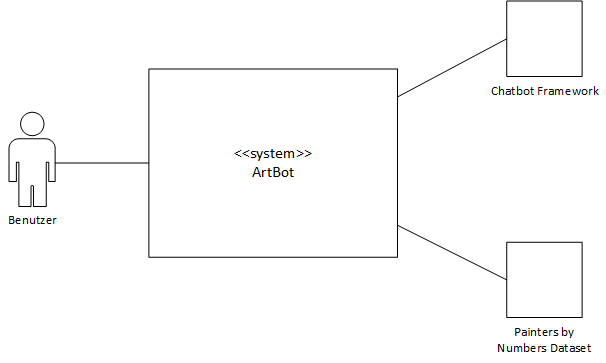
\includegraphics[width=0.6\linewidth]{figures/fachKontext.png}}
	\caption{Fachlicher Kontext von ArtBot}
	\label{fachKontext}
\end{figure}
	
\paragraph{Menschlicher Anwender(Benutzer)}
ArtBot ist ein Chatbot, dessen Funktion es ist, auf Nachfrage Bilder von berühmten Künstlern auszugeben. Dafür muss ein Benutzer mit ArtBot interagieren und über ein Chatfenster die nötigen Informationen eingeben.  

\paragraph{Chatbot Framework - Rasa (Fremdsystem)}
Die Grundlage für den Chatbot bildet ein Framework, hier haben wir uns für Rasa entschieden. Ein Framework vereinfacht die Erstellung des Chatbots, indem es ein Grundgerüst mit den wichtigen Funktionen bereitstellt.

\paragraph{Painter by Numbers (Datensatz)}
Die Grundlage für die Daten des Chatbots bildet ein Datensatz, der auf der Webseite Kaggle.com veröffentlicht wurde. Dieser Datensatz enthält Bilder von berühmten Künstlern zusammen mit diversen Hintergrundinformationen. Dieser Datensatz wird in \ref{daten} genauer beschrieben.
\newpage

\subsection{Technischer Kontext}
\begin{figure}[H]
	\centerline{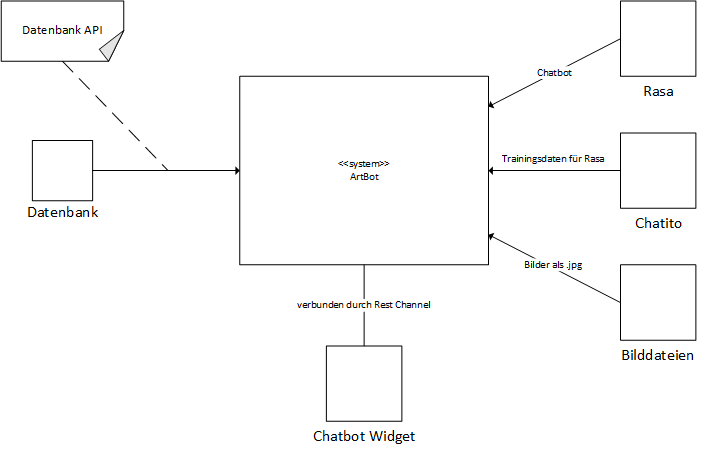
\includegraphics[width=0.9\linewidth]{figures/techKontext.png}}
	\caption{Technischer Kontext von ArtBot}
	\label{techKontext}
\end{figure}

\paragraph{Rasa}
Wie in \ref{fach_text} bereits erwähnt, haben wir uns bei der Wahl unseres Frameworks für Rasa entschieden \cite{rasa_mainpage}. Dabei war wichtig, dass das Framework Open Source ist und es eine solide Grundlage mit guter Erweiterbarkeit bietet. Rasa ist ein Framework für automatisierte Konversationen, welches auf Machine Learning basiert. Der genaue Aufbau von Rasa sowie die Erweiterung werden in späteren Kapiteln detaillierter beschrieben.

\paragraph{Chatito}
Da für Rasa Trainingsdaten und Testdaten benötigt werden und es sehr mühsam ist diese von Hand zu schreiben, haben wir Chatito verwendet, um diese zu generieren. Chatito ist eine Online Anwendung, die unter \cite{chatito_ide} aufrufbar ist. Diese Anwendung erleichtert das Erstellen von Datensätzen ungemein, indem sie aus einigen vom Benutzer eingegebenen Wörtern Datensätze erstellt, welche dann direkt mit Rasa (und auch anderen Frameworks) verwendet werden können. Dieser Vorgang wird in \ref{chatito} genauer beschrieben.

\paragraph{Datenbank}
Die grundlegenden Daten und Bilder die für ArtBot zum Einsatz kommen, entstammen einem Datensatz, welcher in \ref{daten} genauer beschrieben wird. Die Daten dieses Datensatzes haben wir gekürzt und die relevanten Informationen in eine Datenbank geschrieben. Das Modell dieser Datenbank wird in \ref{datenbankmodell} genauer erläutert.

\paragraph{Bilddateien}
Die zu den Daten in der Datenbank zugehörigen Bilder, welche auch aus dem Kaggle Datensatz stammen, sind in einem extra Ordner abgelegt. Diese werden über den Dateinamen, welcher auch in der Datenbank hinterlegt ist, zugeordnet. 

\paragraph{Chatbot Widget}
Da der grundlegende Chatbot, welcher mit Rasa entwickelt wurde, nur auf der Kommandozeile arbeitet, wird ein Frontend benötigt, um Bilder auszugeben. Für diesen Zweck haben wir das Chatbot Widget verwendet. Das ist ein Frontend für Rasa, welches im Browser ausgeführt wird, auf Javascript, HTML sowie CSS basiert und mithilfe von Rest Channels mit Rasa kommuniziert. Dies wird in \ref{chatbot_widget} genauer beschrieben. Dieses Frontend stammt von Jitesh Gaikwad und wurde auf Github unter \cite{chatbot_widget} veröffentlicht.

\subsection{Datengrundlage}\label{daten}
Wie bereits vorher erwähnt, basieren die Daten, welche dem ArtBot zur Verfügung stehen, auf einem Datensatz der auf der Website Kaggle.com veröffentlicht wurde. Der Name des Datensatzes ist Painter by Numbers und er wurde im Rahmen eines Wettbewerbs erstellt. Bei diesem Wettbewerb sollte ein Algorithmus entwickelt werden, der Bilder paarweise überprüft, ob diese vom gleichen Künstler sind. Dafür wurde ein großer Datensatz mit über 2000 Künstlern und über 10000 Bildern sowie zahlreiche Zusatzinformationen bereitgestellt. Dabei war der Datensatz bereits in Trainings- und Testdaten für den Fall des Wettbewerbs aufgeteilt. Der Datensatz ist unter \cite{datensatz} zu finden und die Struktur der Hauptdatei all\_data\_info.csv ist in \ref{datensatz} abgebildet. Für das Projekt waren nur die Hauptdatei, sowie die einzelnen Bilder interessant. Für die Zwecke von ArtBot haben wir zuerst die Attribute date, pixelsx, pixelsy, size\_bytes, source, artist\_group und in\_train entfernt. Zusätzlich wurden alle Einträge entfernt, welche leere Felder beinhalten. Daraufhin haben wir 20 Künstler mit jeweils 5 Bildern ausgewählt und diese als unseren Datensatz für ArtBot gewählt.

\begin{figure}[H]
	\centerline{\includegraphics[width=1.0\linewidth]{figures/datensatz.png}}
	\caption{Aufbau der Hauptdatei all\_data\_info.csv}
	\label{datensatz}
\end{figure}
	\section{Konzept (Joshua Hörmann)}
In diesem Kapitel wird ein Überblick über das Architekturkonzept gegeben und das Datenbankmodell erklärt.
\subsection{Architekturkonzept}
\begin{figure}[H]
	\centerline{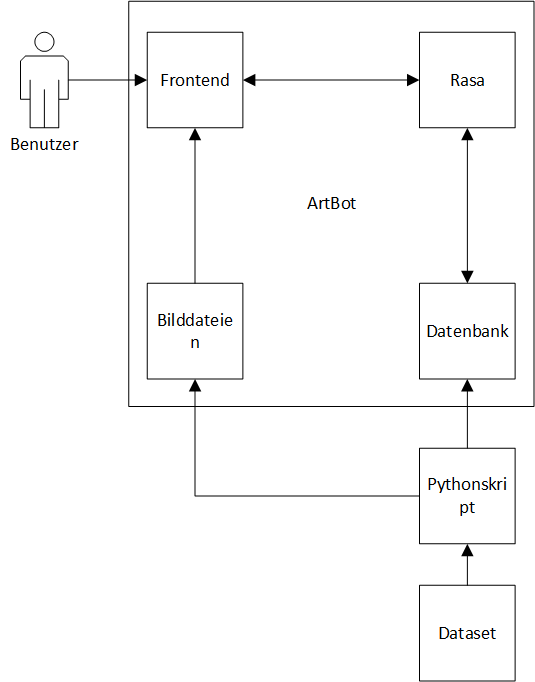
\includegraphics[width=0.6\linewidth]{figures/konzept.png}}
	\caption{Architekturkonzept des ArtBots}
	\label{konzept}
\end{figure}

In Abbildung \ref{konzept} ist das Konzept des ArtBots dargestellt. Dabei interagiert der Benutzer mit einem Frontend, welches mit Rasa verbunden ist und die eingegebenen Befehle an Rasa weitergibt. Rasa bearbeitet diese entweder intern oder stellt eine Anfrage an die Datenbank. Die entsprechende Antwort wird an das Frontend zurückgegeben und dort ausgegeben. Wenn ein Bild zur Ausgabe benötigt wird, holt sich das Frontend die entsprechende Bilddatei über den Dateinamen. Die Datenbank sowie der Ordner mit den Bilddateien werden mithilfe eines Python-Skripts mit Daten aus dem Dataset befüllt. Der Aufbau der fertigen Implementierung ist unter \ref{umsetzung} dargestellt. Im Folgendem wird das Datenbankmodell vorgestellt.

\subsection{Datenbankmodell}\label{datenbankmodell}
Der Aufbau der Datenbank ist simpel gehalten, da wir nur eine vereinfachte Abbildung des Datensatzes benötigt haben. Daher enthält er nur die beiden Tabellen Artists und Pictures. Die Tabelle Artists enthält die Künstler mit ihrem Namen als Primary Key und dem Geburtsdatum als zusätzliches Attribut. Das Geburtsdatum wird noch nicht verwendet, wir haben es aber für die spätere Erweiterbarkeit eingefügt. Die Tabelle Pictures enthält die Eckdaten der einzelnen Bilder. Dabei sind der Dateiname, der Name des Künstlers, der Titel, die Epoche, sowie das Genre abgelegt. Der Filename ist dabei der Primary Key und der Künstlername ein Foreign Key. Dieser Aufbau ist in \ref{datenbank} illustriert. Zuerst hatten wir noch versucht die Bilder ebenfalls in der Datenbank abzulegen, aber da die Datenbank dadurch viel zu groß wurde und es zu Konvertierungsschwierigkeiten beim Einfügen und Auslesen aus der Datenbank kam, haben wir uns gegen diesen Ansatz entschieden. Die Bilder haben wir daraufhin in einen extra Bilderordner abgelegt.

\begin{figure}[H]
	\centerline{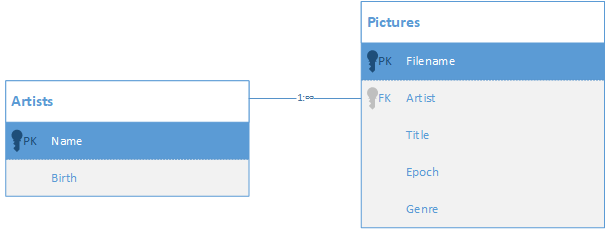
\includegraphics[width=0.7\linewidth]{figures/Datenbankmodell.png}}
	\caption{Darstellung des Datenbankmodells}
	\label{datenbank}
\end{figure}

\newpage


	\section{Implementierung (Joshua Hörmann)}
Dieses Kapitel beschäftigt sich mit der eigentlichen Implementierung des Artbots. Zu diesem Zweck wird zuerst auf die verwendeten Tools \& Libraries eingegangen, um dann die konkrete Umsetzung und den Zusammenhang zu erklären.
\subsection{Tools \& Libraries}
\paragraph{Rasa}
Die Grundlage des ArtBots bildet das Rasa Framework. Rasa ist ein Open-Source Framework, welches zur Entwicklung von Chatbots mithilfe von Machine Learning eingesetzt wird. Dabei ist Rasa in zwei Hauptteile aufgeteilt: Rasa NLU (Natural Language Understanding) und Rasa Core. Dabei kümmert sich Rasa NLU um alles, was Natural Language Processing (NLP) betrifft und extrahiert die wichtigen Aussagen. Daraufhin kümmert sich Rasa Core um das Dialog Management und die Erstellung der Antworten des Chatbots \cite{rasa_definition}. Dies ist nur eine sehr grobe Beschreibung von Rasa, deutlich detaillierter ist es unter \ref{sec:flow} bzw. \cite[S.9f]{seminar} beschrieben.
\paragraph{Chatbot Widget designed for Rasa Bots}\label{chatbot_widget}
Für das Frontend wurde 'Chatbot Widget designed for Rasa Bots' von Jitesh Gaikwad verwendet \cite{chatbot_widget}. Dies ist ein Open Source Frontend, welches mit Javascript programmiert ist und sich leicht in Webseiten einbinden lässt. Es kommuniziert mit Rasa über sogenannte REST Channels. REST steht für Representational State Transfer und ist ein geläufiges Konzept für APIs. Dabei stellt der Rasa-Bot eine URL bereit, an welche das Chatbot Widget Requests senden kann und basierend darauf schickt Rasa dann einen entsprechenden Response an das Chatbot Widget zurück. \cite{rest}
\paragraph{Chatito}\label{chatito}
Um das Erstellen von Trainings- und Testdaten zu vereinfachen wurde Chatito verwendet. Chatito ist ein Projekt von Rodrigo Pimentel, welches eine Online Entwicklungsumgebung auf Github bereitstellt. \cite{chatito_ide} In dieser Online IDE kann man mit wenigen Eingaben in einer leicht verständlichen Syntax Datensätze erstellen. Diese Datensätze werden als JSON-Files ausgegeben, können also nicht nur mit Rasa sondern auch mit anderen Frameworks verwendet werden. Mehr zu der Funktionsweise von Chatito kann unter \cite{chatito_spec} nachgelesen werden.
\subsection{Umsetzung}\label{umsetzung}

\begin{figure}[H]
	\centerline{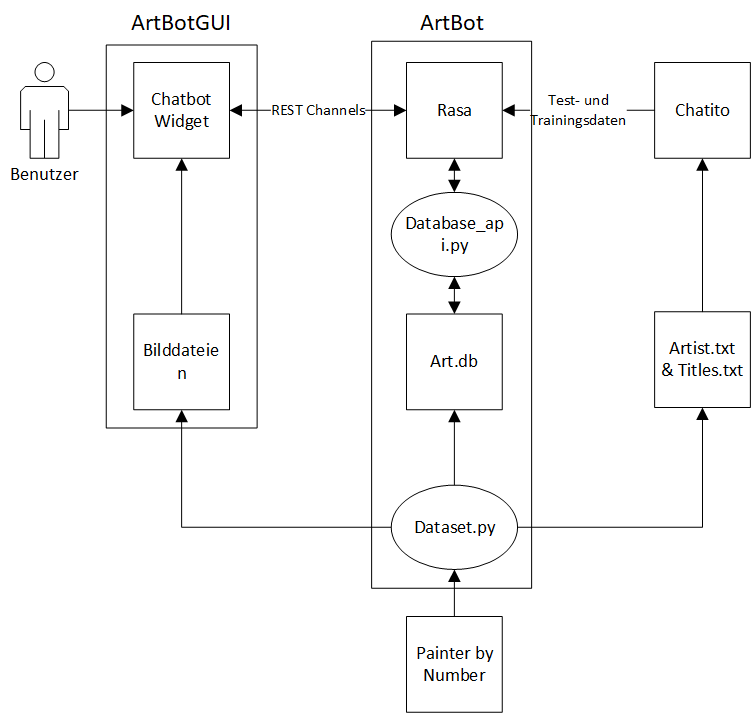
\includegraphics[width=0.8\linewidth]{figures/implementierung.png}}
	\caption{Der Aufbau und die Interaktion des ArtBots}
	\label{img:implemenatation}
\end{figure}

Die Abbildung \ref{img:implemenatation} gibt einen Überblick über den Aufbau und die Interaktionen innerhalb der entwickelten Anwendung. Ebenso kann man anhand der Abbildung die Struktur des Projekts sehen. Der Benutzer interagiert mit dem Chatbot Widget, welches zusammen mit den Bilddateien die ArtBotGUI bildet. Hierbei liegen die Bilddateien innerhalb von \textbackslash ArtBotGUI\textbackslash static\textbackslash art. In dem Ordner ArtBotGUI sind alle weiteren Dateien des Chatbot Widgets abgelegt. Diese GUI interagiert über REST Channels mit dem Rasa Chatbot, der mit der Datenbank Art.db, der Datenbank API Database\_api.py und dem Pythonscript Dataset.py zum Erstellen der Datenbasis den ArtBot bildet. All diese Dateien befinden sich in dem Ordner ArtBot, zusätzlich sind hier diverse Dateien von Rasa vorhanden, wie zum Beispiel die Testdaten in train\_test\_split oder die config.yml. Außerhalb des ArtBots und der GUI befindet sich der Datensatz, woraus mithilfe von Dataset.py die Datenbank und die Bilddateien extrahiert werden. Zusätzlich erzeugt dieses Pythonprogramm noch die zwei Textdateien Artist.txt und Titles.txt, welche zum Erstellen der Trainings- und Testdaten in Chatito benötigt werden. Die von Chatito erzeugten Datensets werden dann wiederum in Rasa innerhalb des ArtBots für das Training verwendet. 

	\section{ArtBot's Workflow (Fabio Aubele)}\label{sec:flow}
Der grundlegende Arbeitsablauf des entwickelten Chatbot ist bereits von Rasa vorgegeben. Grafik \ref{flow} beschreibt diesen genauer.
\begin{figure}[htbp]
	\centerline{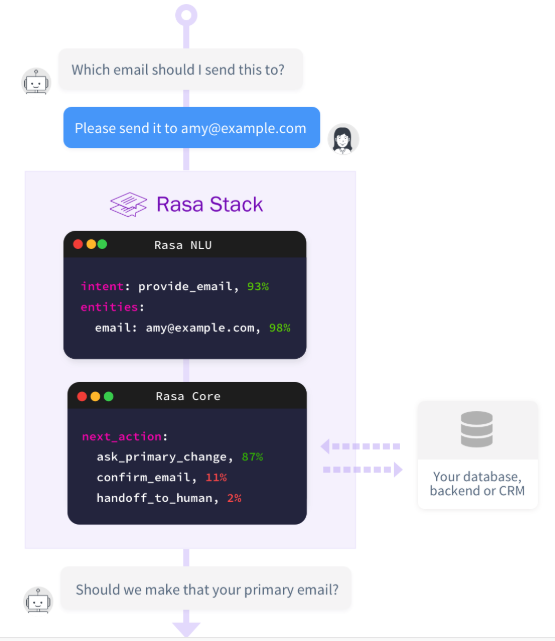
\includegraphics[width=1\linewidth]{figures/rasa_full.jpg}}
	\caption{Genereller Workflow von ArtBot.}
	\label{flow}
\end{figure}
Zunächst ist nur die Äußerung des Benutzers vorhanden. Diese wird dann von Rasa NLU verarbeitet, als Ergebnis werden Intent und Entities ausgegeben. Daraufhin werden diese von Rasa Core benutzt, um die nächste auszuführende Aktion des Chatbots zu ermitteln. Dies können normale textuelle Äußerungen sein, welche einfach wiedergegeben werden oder es wird externer Python-Code aufgerufen. Innerhalb der entwickelten Anwendung führt dieser Code immer Datenbankabfragen aus, womit überprüft wird, ob der von dem Benutzer genannte Maler oder das genannte Kunstwerk in der Datenbank vorhanden ist. Falls dies zutrifft, wird das gewünschte Kunstwerk angezeigt. Hierbei gibt es unterschiedliche Möglichkeiten für den Benutzer, nach einem Bild zu fragen. Diese sind dabei in Kapitel \ref{sec:dialog} aufgezeigt. Die nächsten beiden Kapitel erklären die Arbeitsabläufe in Rasa NLU und Rasa Core genauer. Um den grundlegenden Aufbau und alle Begrifflichkeiten rund um Rasa zu verstehen, empfiehlt es sich, davor die dazugehörige Seminar-Arbeit (Quelle \cite[S.9-11]{seminar}) durchzulesen.

\subsection{Rasa NLU}\label{sec:flownlu}
Rasa NLU transformiert die Äußerung des Benutzers in einen jeweiligen Intent und endlich vielen Entities. Um diesen Schritt zu ermöglichen, müssen erstmals alle nötigen Intents und Entities angegeben werden. Dies geschieht durch eine Markdown- oder Json-Datei in der von Rasa vorgegebenen Formatierung.\\
Um die Umwandlung zu vollziehen, benötigt es die sogenannte Pipeline von Rasa. Diese setzen sich aus mehreren Komponenten zusammen, welche allesamt zusammenarbeiten. Der Kernbestandteil ist ein Machine Learning Algorithmus, welcher die gewünschten Entities erkennt und ein neuronales Netz, welches die Sätze mit dem jeweils korrekten Intent klassifiziert. Rasa bietet dabei vorkonfigurierte Pipelines an, die für häufig vorkommende Use-Cases optimiert sind. Eine Übersicht der einzelnen Bestandteile und der vorkonfigurierte Pipelines bietet Quelle \cite{nlunn} an.\\
\\
Innerhalb dieser Arbeit wurde die vorkonfigurierte Pipeline 'supervised\_embeddings' verwendet. Diese ermöglicht es, Anwendungen in anderen Sprachen (der Standard ist Englisch) zu formulieren und da der entwickelte Chatbot nur auf deutsche Angaben reagieren soll, eignet sich diese Pipeline optimal. Die einzelnen Bestandteile sind in Abbildung \ref{se} aufgelistet.
\begin{figure}[htbp]
	\centerline{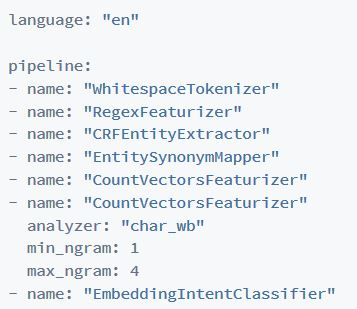
\includegraphics[width=0.5\linewidth]{figures/se.jpg}}
	\caption{Bestandteile der 'supervised\_embeddings' Pipeline \cite{nlunn}.}
	\label{se}
\end{figure}
Die angegebene Sprache in der ersten Zeile wurde für ArtBot in 'de' für deutsch abgeändert. Der nun erste Teil der Pipeline ist der 'WhitespaceTokenizer', welcher die einzelnen Wörter der Äußerung des Nutzers anhand von Leerzeichen trennt. Darauf folgt der 'RegexFeaturizer', der benötigt wird, um reguläre Ausdrücke zu erkennen. Dies wird in dieser Anwendung jedoch nicht benutzt. Nun folgt der 'CRFEntityExtractor', welcher einer der wichtigsten Bestandteil der Pipeline ist, da sich dieser um die Extraktion der Entities kümmert. Hierbei wird ein Conditional Random Field (CRF) Model aus der Python-Bibliothek 'scikit-learn'\footnote{siehe \href{https://scikit-learn.org/stable/}{https://scikit-learn.org/stable/}} verwendet \cite{nlunn}. Ein CRF-Model ist ein 'Discriminative Model', welches zum Erkennen von Pattern eingesetzt wird und somit häufig benutzt wird, um Vorhersagen in sequenziellen Daten zu treffen \cite{crf}. Dabei werden kontextuelle Informationen benötigt. Dies ist auch der Grund, dass sich dieser Algorithmus sehr gut eignet, um Entities zu erkennen, da diese stark von den vorherigen und nachfolgenden Wörtern abhängen. Eine detaillierte Erklärung des CRF-Model bietet Quelle \cite{crf} an.\\
Der nächste Bestandteil ist der 'EntitySynonymMapper', mit dessen Hilfe den Entities Synonyme zugeordnet werden können. Dies wird allerdings in der entwickelten Anwendung ebenfalls nicht verwendet. Dann folgen zwei 'CountVectorsFeaturizer', welche Merkmale aus den gegebenen Wörtern ableiten, die von dem 'WhitespaceTokenizer' extrahiert worden sind. Anhand dieser Merkmale kann der nächste Teil der Pipeline die vorliegende Klassifizierungsaufgabe lösen. Der erste 'CountVectorsFeaturizer' benötigt dafür nur die extrahierten Wörter. Die zweite Instanz benutzt N-Gramme, welche die einzelne Buchstaben der Wörter neu zusammenfügt und dann die Erzeugnisse zum Erstellen von Merkmalen anwendet. Die darunter stehenden Argumente sind die Einstellungen, welche zur Erzeugung der N-Gramme verwendet werden. Diese geben die minimale (1) und maximale Länge (4) an, sowie die eingesetzte Methode (char\_wb), welche angibt, dass nur Zeichen innerhalb der definierten Grenze hergenommen werden dürfen. Für eine genauere Erklärung von N-Grammen siehe Referenz \cite{ngramm}.\\
\\
Zu guter Letzt folgt der 'EmbeddingIntentClassifier', welcher der wichtigste Teil der Pipeline ist, da dieser die Klassifizierungsaufgabe löst und den finalen Intent ausgibt. Dieser benutzt ein neuronales Modell namens StarSpace, welches in Quelle \cite{starspace} detailliert vorgestellt wird. Dabei werden die durch den 'CountVectorsFeaturizer' erstellten Merkmale benötigt, um dem gegebenen Satz den korrekten Intent zuzuordnen. Der Aufbau des neuronalen Netzes ist in Abbildung \ref{star} zu sehen.
\begin{figure}[htbp]
	\centerline{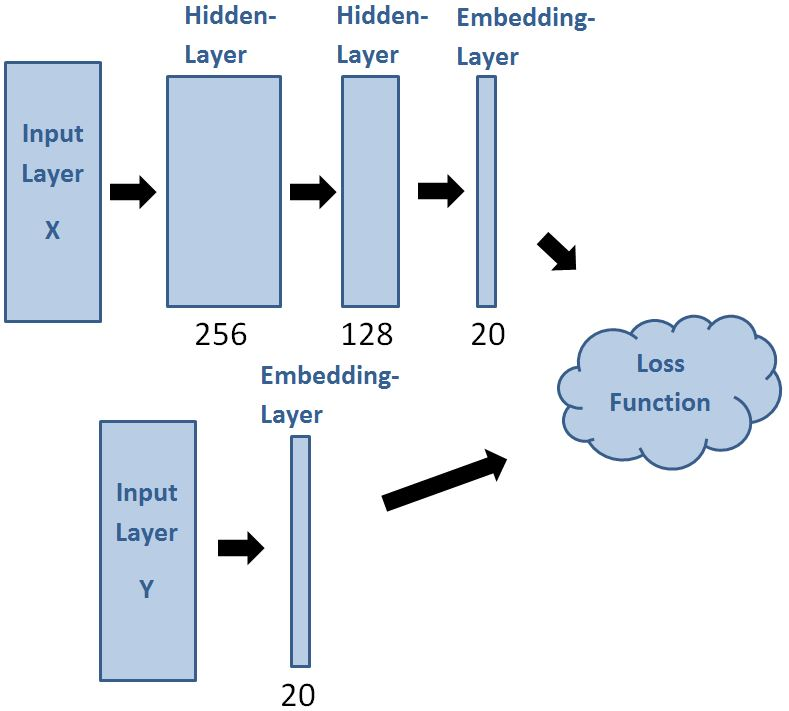
\includegraphics[width=0.8\linewidth]{figures/star.jpg}}
	\caption{Aufbau des neuronalen Netzes zur Intent-Erkennung (basierend auf \cite{ftech}).}
	\label{star}
\end{figure}
Dabei gibt es zwei getrennte Netze, eines für die Eingabe des Benutzers (X) und eines für die definierten Intents (Y), welche als Label verwendet werden. Die Eingaben des Benutzers werden durch zwei Hidden-Layers geführt, mit 256 Neuronen und 128 \cite{ftech}. Daraufhin folgt der Embedding Layer (20 Neuronen), welche die Buchstaben in einen Zahlenvektor umwandelt. Die Intents werden nur durch den Embedding Layer geführt \cite{ftech}. Zuletzt wird mittels einer Loss-Function die Unähnlichkeit der Ergebnisse beider Embedding Layers bestimmt. Dafür wird die Kosinus-Ähnlichkeit benutzt \cite{ftech}. Der am wenigsten unähnliche Intent wird als Klassifizierungsergebnis bestimmt.\\
\\
Mithilfe dieses Vorgehens lässt sich das neuronale Netz trainieren, um die optimalen Gewichte zwischen den einzelnen Layern zu finden. Daraufhin kann das Netz später eingesetzt werden, um den Äußerungen des Nutzers einen Intent zuzuordnen. Die Intents müssen dabei vorher bereits definiert worden sein, um das Netz für diese zu trainieren. Rasa ermöglicht dem Entwickler bestimmte Einstellungen des Netzes zu ändern und anzupassen, innerhalb von ArtBot werden jedoch die Standard Einstellungen benutzt. Eine Übersicht der Standardeinstellungen und aller änderbaren Eigenschaften sind in Quelle \cite{embedd} aufgelistet.\\
Final erhält die Anwendung durch diese Pipeline und somit durch Rasa NLU den Intent und die verwendeten Entities innerhalb einer Äußerung des Benutzers.

\subsection{Rasa Core}\label{sec:flowcore}
Rasa Core verwendet den gegebenen Intent und die gegebenen Entities, um die nächste Aktion des Chatbots zu ermitteln. Dabei wird unterschieden zwischen 'utterance-actions', was normale textuelle Äußerungen des Chatbots sind und 'custom-actions', welche externe Logik mit Hilfe von Python-Code ausführen. Für die entwickelte Anwendung ArtBot werden 'custom-actions' nur benötigt, um Eingaben zu überprüfen sowie aus der anhängenden Datenbank Informationen zu holen und diese auszugeben.\\
Um diese Funktionalität zu ermöglichen, müssen vorerst sogenannte Stories angelegt werden. Diese widerspiegeln den Gesprächsfluss des Benutzers und des Chatbots. Definiert werden diese in einer von Rasa vorgegebenen Form innerhalb von Markdown-Dateien. Zusätzlich fungieren diese Stories als Trainingsdaten für die Policies.\\
\\
Rasa Core verwendet Policies, um die nächste auszuführende Aktion des Chatbots algorithmisch zu ermitteln. Nun gibt es mehrere vorkonfigurierte Policies für verschiedene Anwendungsfälle. In der entwickelten Anwendung ArtBot wurden folgende benutzt:
\begin{itemize}
	\setlength\itemsep{-0.6em}
	\item MemoizationPolicy
	\item MappingPolicy
	\item KerasPolicy
\end{itemize}
Die MemoizationPolicy sagt die nächste Aktion mit einer Wahrscheinlichkeit von 1.0 vorher, wenn die Konversation mit dem aktuellen Nutzer mit einer Konversation aus den Trainingsdaten übereinstimmt. Hierbei merkt sich die Policy die Konversationen aus den Trainingsdaten und vergleicht diese dann. Gibt es keine Übereinstimmungen wird None (Datentyp in Python) vorhergesagt mit einer Wahrscheinlichkeit von 0.0. Tritt dieser Fall ein, wird sich auf das Ergebnis der anderen Policies verlassen.\\
Etwas anders funktioniert die MappingPolicy, welche die Trainingsdaten nicht benötigt. Hier muss bei der Definition eines Intents innerhalb der Domain das Attribut 'triggers' verwendet werden, ansonsten wird diese Policy nicht ausgelöst. Ein Beispiel dafür ist in Code \ref{trigger} zu sehen.
\begin{lstlisting}[caption={Verwendung der MappingPolicy innerhalb von ArtBot.}, label=trigger, lineskip=1pt, morekeywords={intents, greet, goodbye}]
intents:
  - greet:
    triggers: action_greet
  - goodbye:
    triggers: utter_goodbye
...
\end{lstlisting}
Durch dieses Konstrukt löst der Intent \texttt{greet} nun immer \texttt{action\_greet} aus, was eine 'custom-action' ist und der Intent \texttt{goodbye} immer \texttt{utter\_goodbye}, was wiederum eine 'utterance-action' ist.\\
\\
In den meisten Fällen wird jedoch die KerasPolicy angewendet, welche die gleichnamige Python-Bibliothek Keras\footnote{siehe \href{https://keras.io/}{https://keras.io/}} benutzt. Dafür wird ein neuronales Netz mit der Long Short Term Memory (LSTM) Architektur verwendet, welches ein Recurrent Neural Network (RNN) ist. LSTM's haben die Möglichkeit langfristige Abhängigkeiten festzuhalten. Dabei werden sich Informationen gemerkt und für spätere Zusammenhänge wiederverwendet. Diese Eigenschaft ist für Chatbots besonders wichtig, da der Gesprächsverlauf auch durch frühe Dialogentscheidungen beeinflussbar sein muss. Eine detaillierte Erklärung der LSTM Architektur und seiner Eigenschaften bietet Quelle \cite{lstm}. In Rasa soll der Dialog durch folgende drei Faktoren zusätzlich beeinflussbar sein \cite{rasa}:
\begin{itemize}
	\setlength\itemsep{-0.6em}
	\item Was war die letzte Aktion des Chatbots?
	\item Was ist der Intent und die Entities der letzten Nachricht des Benutzers?
	\item Welche Slots sind momentan belegt?
\end{itemize} 
Um dies zu realisieren benötigt es die in Abbildung \ref{lstm} vereinfacht beschriebene Architektur.
\begin{figure}[htbp]
	\centerline{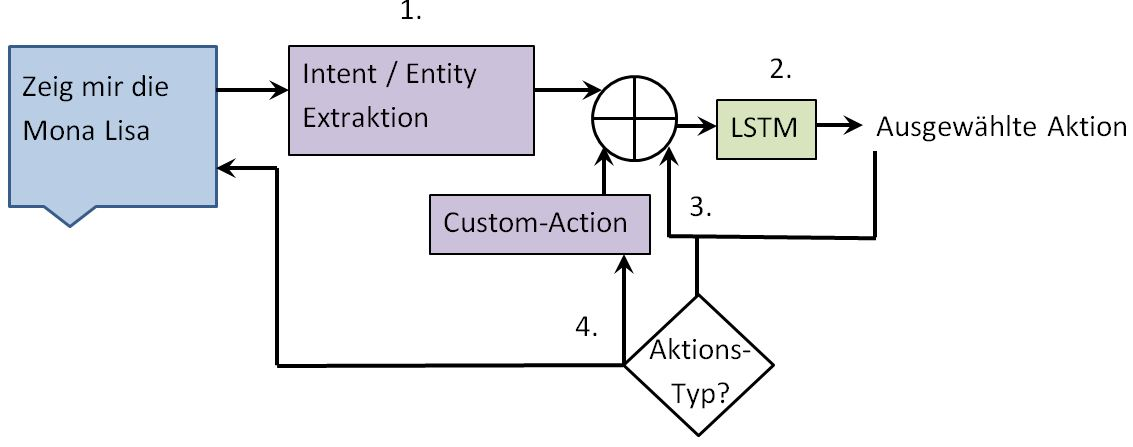
\includegraphics[width=1\linewidth]{figures/lstm.jpg}}
	\caption{Aufbau von LSTM in Rasa Core (basierend auf \cite{lstmrasa}).}
	\label{lstm}
\end{figure}
\\Zunächst werden in Schritt eins Intent und Entity durch Rasa NLU extrahiert. Daraufhin folgt der Aufruf von LSTM in Schritt zwei. Hier nimmt LSTM nicht nur Rücksicht auf den momentanen Intent und die momentanen Entities, sondern auch auf die vorherigen aufgerufenen Aktionen, welche sich für weitere Vorhersagen gemerkt werden (dargestellt durch den Kreis) \cite{lstmrasa}. LSTM wählt anhand dieser Informationen und den als Trainingsdaten verwendeten Stories nun die nächste Aktion aus. Daraufhin wird diese in Schritt 3 wieder als Information für den nächsten Aufruf hinterlegt (Kreis) \cite{lstmrasa}, damit LSTM weiterhin die zuletzt ausgeführte Aktion kennt. Dann wird in Schritt 4 entschieden, was für ein Typ die von LSTM ausgewählte Aktion ist \cite{lstmrasa}. Bei einer 'custom-action' wird der entsprechende Python-Code aufgerufen und ausgeführt. Hier kann es sein, dass die 'custom-action' zusätzliche Aktionen ausführt oder Slots abändert. Dies wird daraufhin wieder als Information hinterlegt (Kreis). Ist die Aktion jedoch eine 'utterance-action' wird der Text nur ausgegeben. Es kann auch passieren, dass die ausgewählte Aktion in Schritt 2 lediglich einen Slot abändert. Dies wird ebenfalls für den nächsten Aufruf hinterlegt (Kreis), jedoch folgt keine Ausgabe von Text oder die Ausführung einer 'custom-action'.\\
Für eine noch detaillierte Erklärung der Verwendung von LSTM innerhalb von Rasa steht Quelle \cite{lstmrasa} zur Verfügung. Wie genau LSTM aufgebaut ist und wie groß das dadurch aufgespannte Netz ist, wurde von Rasa nicht dokumentiert.\\
Rasa Core ermöglicht somit, die korrekte Aktion des Chatbots für eine Äußerung des Nutzers zu ermitteln und diese auszuführen, wie in den Stories vermerkt. Zusammen mit Rasa NLU und der implementierten Datenbank-API wird somit der in Abbildung \ref{flow} dargestellte Workflow realisiert.

\subsection{Gesprächsfälle}\label{sec:dialog}
Bei der Erstellung der Trainingsdaten, mit welchen die in den Kapiteln \ref{sec:flownlu} und \ref{sec:flowcore} beschriebenen Netze trainiert werden, wurde darauf geachtet, dass es dem Chatbot möglich ist, auf mehrere unterschiedliche Gesprächsfälle einzugehen. Diese sollen in diesem Abschnitt erläutert werden. Auch wurde ein Teil der Logik innerhalb der 'custom-actions' implementiert. Hier wird geprüft, ob die Angaben zu Künstler und Kunstwerk korrekt sind und in der Datenbank auch vorkommen. Wie bereits erwähnt, ist der generelle Anwendungsfall Bilder anzuzeigen, nachdem der Künstler und das Kunstwerk von dem Benutzer genannt wurde.\\
\\
Grundlegend kann für den Künstler immer der volle Name oder nur der Vorname bzw. der Nachname angegeben werden. Gibt es dabei mehrere Künstler, welche zum Beispiel den selben Vornamen haben, werden alle in Frage kommende Künstler aufgelistet (z.B. bei Paul: Paul Gauguin, Paul Cezanne und Peter Paul Rubens), damit der Benutzer einen davon in der nächsten Eingabe auswählen kann. Das gleiche gilt auch für Kunstwerke. Hier kann der volle Titelname genannt werden, welcher in dem benutzten Datensatz immer einzigartig ist oder nur der Anfang eines Titels (z.B. 'Resurrection' für 'Resurrection of Lazarus'). Gibt es mehrere Bilder mit dem selben Anfang, werden alle aufgelistet (z.B. Portrait: 'Portrait of a Young Man' oder 'Portrait of Gaspard Schoppins'), damit der Benutzer wieder eines auswählen kann. Falls der Benutzer nicht den exakt korrekten Titel des Kunstwerkes oder Namen des Künstlers nannte, gibt der Chatbot innerhalb einer Extra-Ausgabe den jeweils korrekten Wert an.\\
\\
Nun gibt es drei mögliche Fälle, auf welcher Art der Benutzer nach einem Kunstwerk fragen kann: 
\begin{enumerate}
	\setlength\itemsep{-0.6em}
	\item Der Benutzer nennt Künstler und Kunstwerk in einer Äußerung.
	\item Der Benutzer nennt erst den Künstler in einer Äußerung und daraufhin das Kunstwerk.
	\item Der Benutzer nennt nur das Kunstwerk in einer Äußerung.
\end{enumerate}
Für den ersten Fall müssen sowohl der Künstler, als auch das Kunstwerk in der Datenbank vorhanden sein. Ansonsten wird angegeben, welcher Wert falsch war. Sind beide Werte korrekt wird das Bild angezeigt.\\
Innerhalb des zweiten Falles nennt der Nutzer zuerst den Künstler, welcher wiederum in der Datenbank stehen muss oder es wird angegeben, dass der Künstler nicht vorhanden ist. Daraufhin wird dem Benutzer eine Auswahl der zur Verfügung stehende Kunstwerke dieses Künstlers aufgelistet. Hier kann der Benutzer nun eines dieser Werke auswählen, wenn der Benutzer das Kunstwerk korrekt wiedergibt und es somit in der Datenbank vorhanden ist, wird es daraufhin angezeigt. Nach dem Benennen eines Künstlers muss der Benutzer kein Kunstwerk angeben, er kann auch je nach Belieben wieder einen der drei oben genannten Fälle auslösen.\\
Für den letzten Fall kann der Benutzer nur den Titel eines Kunstwerkes nennen, welches sofort angezeigt wird, wenn es in der Datenbank vorhanden ist. Ansonsten gibt ArtBot an, dass ein solches Kunstwerk nicht existiert. Hier kann auch der Fall auftreten, dass der Titel zu ungenau ist, dabei werden, wie oben erwähnt, alle in Frage kommende Bilder aufgelistet.\\
\\
Diese Modellierung der Gesprächsfälle erlaubt es auch, nur einen Intent anlegen zu müssen, was die Implementation erleichtert. Eine Fallunterscheidung kann gemacht werden, indem geprüft wird, wie viele Entities der Nutzer angegeben hat. Dies wird von Rasa unterstützt, wodurch kein zusätzlicher Programmieraufwand entsteht. Insbesondere bei ähnlichen Äußerungen schlägt Rasa ein solches Vorgehen sogar vor. Dies bedeutet für Fall 1 werden beide Entities (Künstler und Titel des Kunstwerkes) benötigt, für Fall 2 nur der Künstler und bei Fall 3 nur der Titel des Kunstwerkes.

	\section{Erweiterungen (Fabio Aubele)}\label{sec:erweiterungen}
Da ArtBot nur innerhalb eines Semesters geplant, implementiert und dokumentiert wurde, gibt es viele Möglichkeiten, wie das Projekt zusätzlich ergänzt werden kann. Innerhalb dieses Abschnittes soll dabei zunächst auf mögliche Verbesserungen und zusätzliche Funktionen der Anwendung eingegangen werden. Daraufhin wird eine Anleitung geschildert, mit dessen Hilfe der Chatbot um weitere Logik ergänzt werden kann.

\subsection{Verbesserungen und zusätzliche Funktionalitäten}
Die entwickelte Anwendung kann mit vielen Verbesserungen ergänzt werden. Zunächst wäre die generelle Architektur der 'custom-actions' zu nennen. Momentan gibt es für jeden der drei Gesprächsfälle aus Kapitel \ref{sec:dialog} eine 'custom-action'. Diese holt sich anhand der Eingabe vom Benutzer die Informationen aus der Datenbank. Je nachdem welche und wie viele Daten zurückgegeben wurde, was wiederum signalisiert, ob die Eingabe des Benutzers korrekt war, wird eine Ausgabe des Chatbots ausgelöst. Eine weitaus sauberere Möglichkeit wäre es jedoch, für jeden Fall zwei 'custom-actions' zu implementieren. Die erste holt sich die Daten aus der Datenbank und die zweite kümmert sich um die Ausgabe. Somit wäre mehr Rücksicht auf das Prinzip 'Separation of Concerns' genommen, was zur Übersicht und Qualität des Codes beitragen würde.\\
\\
Eine der wichtigsten Verbesserungen wäre das Hinzufügen von Small-Talk. Dies würde erlauben, dass der Chatbot auf ganz alltägliche Kommunikationen mit der richtigen Antwort reagieren kann. Dies kann folgende Fragen miteinbeziehen: "Wie geht es dir?", "Wie ist das Wetter heute?", "Wo kommst du her\shorthandoff{"}?" oder \shorthandon{"}"Bist du ein Mensch?". Wichtig dabei ist, dass der Chatbot mit der richtigen Strategie antwortet. Hierbei sollte der Bot also immer auf das Thema Künstler und Kunstwerke hinleiten, dies allerdings nie so abrupt, dass der Benutzer sich übergangen fühlt. Für diese Ergänzungen kann auch die Anleitung unter Kapitel \ref{sec:logik} dienen.\\
\\
Eine weitere Verbesserung würde das Hinzufügen von Stemming und Lemmatization erlauben. Stemming ermöglicht es einzelne Wörter auf ihren Stamm zu reduzieren. Hierdurch wird erreicht, dass verschiedene Formen des selben Wortes nur durch einen Stamm dargestellt werden \cite{stemming}, wie in Abbildung \ref{stemm} mit einem englischen Wortbeispiel zu sehen ist.
\begin{figure}[htbp]
	\centerline{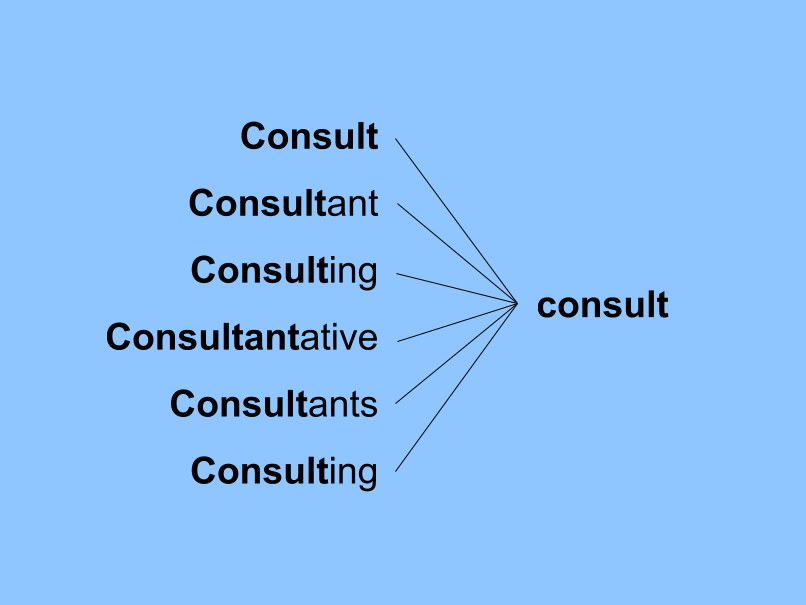
\includegraphics[width=0.5\linewidth]{figures/stemm.png}}
	\caption{Stemming des englischen Wortes 'consult' \cite{stemming2}.}
	\label{stemm}
\end{figure}
Dem entwickelten Chatbot würde dies ermöglichen, auch Eingaben des Nutzers zu verstehen, welche eventuell falsch geschrieben worden sind \cite{stemming}. Innerhalb der entwickelten Anwendung ArtBot müssten die Trainingsdaten, welche die Eingaben des Benutzers widerspiegeln und für Rasa NLU verwendet werden, mithilfe von Stemming abgeändert werden. Daraufhin müsste das neuronale Netz mit den neuen Daten trainiert werden. Dadurch wäre die Erkennung der Eingaben deutlich robuster und zusätzlich wird Redundanz bei der Formulierung der Trainingsdaten verhindert \cite{stemming}.\\
Lemmatization erweitert den eben geschilderten Grundgedanken von Stemming, dabei gilt es nicht nur den Wortstamm zu finden, sondern die wirkliche Normalform des Wortes \cite{stemming}, hier ein Beispiel für ein konjugiertes Verb:\\
sehen, siehst, sah,... -> Normalform: sehen\\
Dies würde dem Chatbot helfen, auch Sätze welche womöglich konjugiert worden sind, korrekt zu erkennen. Zur Umsetzung kann das nltk-Paket\footnote{siehe \href{https://www.nltk.org/}{https://www.nltk.org/}} (Natural Language Tool Kit) in Python benutzt werden, eine Anleitung dafür bietet Referenz \cite{stemming}.\\
\\
Um die Qualität des Chatbots zu erweitern, könnte eine zusätzliche KI-Komponente entwickelt werden. Hier wäre es möglich, das Gespräch mit dem Benutzer genauer zu analysieren. Hat es der Nutzer hierbei nicht innerhalb von ca. 10 Eingaben geschafft, ein Bild auszugeben (Hauptfunktion des Bots) kann eine zusätzliche Ausgabe angezeigt werden, welche die Funktion und die gewünschten Eingaben genau erklärt.\\
Zusätzlich wäre es eine Verbesserung, die Gespräche von ArtBot zu loggen und aus den Log-Dateien neue Daten abzuwandeln, mit welchen der Chatbot wiederum trainiert werden kann. Somit würde der Chatbot durch seine eigenen Konversationen lernen.\\
\\
Die letzte Ergänzung beschreibt eine aufwändigere Änderung. Jedoch wäre es möglich, den Benutzer die Antwort des Chatbots bewerten zu lassen. Dies könnte mit einem Daumen runter Daumen hoch Prinzip realisiert werden. Hierfür müsste für jede Ausgabe des Bots die Wertung des Benutzers zusätzlich mitgeloggt werden. Auch die vorhandene GUI müsste mit neuen Bedienelementen ergänzt werden. Daraufhin lässt sich anhand der erzeugten Daten analysieren, bei welchen Eingaben der Bot eventuell Schwächen aufweist und wo Verbesserungspotenzial besteht.

\subsection{Erweitern der Chatbot-Logik}\label{sec:logik}
Nun soll beschrieben werden, wie die Chatbot-Logik ergänzt werden kann. Zuerst ist zu erwähnen, dass es prinzipiell immer möglich ist, für die momentan bestehenden Gesprächsfälle mehr Vorlagen als Trainingsdaten zu erstellen. Dies würde erlauben, dass auch bei sehr unterschiedlichen Formulierungen des Benutzers die selben Ausgaben zur Verfügung stehen und somit der Chatbot eine konstant bessere Leistung aufzeigt. Innerhalb dieses Kapitels soll jedoch hauptsächlich erklärt werden, wie es möglich ist die Logik des Chatbots zu ergänzen und somit zu erlauben, dass der Bot auch auf andere Gesprächsfälle Bezug nimmt.\\
Hierbei müssen zwei Fälle unterschieden werden. Der erste betrifft Änderungen, welche nur auf eine einfache textuelle Ausgabe des Bots abzielen und der zweite Fall ist für Änderungen, welche externe Logik benötigen. Innerhalb von ArtBot werden dabei meist immer Informationen aus der Datenbank benötigt.\\
\\
Für den ersten Fall muss zunächst ein neuer Intent angelegt werden, welches die potenziellen Eingaben des Nutzers auflistet. Ebenfalls muss der Intent innerhalb einer Story vorkommen mit der entsprechenden Antwort des Bots. Die genaue Syntax des Intents und der Story ist in der Seminararbeit in Quelle \cite[S.10]{seminar} genauer beschrieben. Nun muss noch die Antwort des Chatbots definiert werden. Dies geschieht innerhalb der Domain-Datei (\textit{domain.yml}), wie in Code \ref{domain} zu sehen ist.
\begin{lstlisting}[caption={Einfügen einer neuen Antwort des Chatbots.}, label=domain, lineskip=1pt,
morekeywords={actions, templates, text}]
actions:
  - utter_goodbye
...
templates:
  utter_goodbye:
    - text: Auf Wiedersehen!
    - text: Machs gut!
    - text: Bis bald!
...
\end{lstlisting}
Hierbei muss unter \texttt{actions} nur der generelle Name aufgelistet werden, welcher bei einer textuellen Antwort der Konvention nach mit \texttt{utter\_} anfängt. Unter \texttt{templates} muss dann für jede Antwort der auszugebende Text angegeben werden. Bei mehreren Angaben wird eine zufällig ausgewählt, was bei häufig vorkommende Antworten für mehr Vielfalt sorgt. Wurde alles entsprechend geändert, müssen nun die neuronalen Netze neu trainiert werden, da sich die Trainingsdaten durch das Hinzufügen eines neuen Intent und einer neuen Story geändert haben. Dies geschieht mit der Eingabe \texttt{rasa train} in der Kommandozeile, welche innerhalb der Quelle \cite{command} unter 'Train a Model' genauer beschrieben ist. Daraufhin kann der Bot auf die neue Benutzer-Eingabe mit dem gewünschten Verhalten reagieren.\\
\\
Der zweite Fall benötigt mehr Änderungen. Hier muss ebenfalls ein neuer Intent und eine neue Story angelegt werden. Jedoch wird hier keine einfache textuelle Antwort des Chatbots gebraucht, sondern es wird eine neue 'custom-action' benötigt. Diese muss auch in der Domain-Datei allerdings nur unter \texttt{actions} erwähnt werden, wie in Code \ref{domain} oben zu sehen ist. Die Konvention dabei ist, dass diese mit \texttt{action\_} angeführt werden. Grundlegend wird jede 'custom-action' durch eine eigene Klasse in einer eigenen Python-Datei repräsentiert. Die grundlegende Struktur dieser Klasse und der Datei ist immer gleich. Ein Beispiel ist in Code \ref{custom} zu sehen.
\begin{lstlisting}[caption={Beispiel für den Aufbau einer 'custom-action'.}, label=custom, lineskip=1pt,showlines=true]
from rasa_sdk import Action, Tracker
from rasa_sdk.executor import CollectingDispatcher
from rasa_sdk.events import SlotSet

import database_api as api

class ActionFetchArt(Action):

  def name(self):
    return "action_fetch_art"

  def run(self, dispatcher: CollectingDispatcher, tracker: Tracker, 
          domain: Dict[Text, Any]):
    # get slots
    user_art = tracker.get_slot('art')
    # get images from database
    images = api.get_pictures_by_title(user_art)
	...
    # output a message
    dispatcher.utter_message("Hier das gewünschte Bild!")
    # set slot back to default
    return [SlotSet("art", None)]
    
\end{lstlisting}
Zunächst benötigt es einige Dateien der Bibliothek Rasa, welche importiert werden. Zusätzlich ist auch die Datenbank-API bereits importiert worden (Zeile 5). Daraufhin wird eine Klasse erstellt, welche die 'custom-action' widerspiegelt. Hierbei sind zwei Methoden Pflicht. Die erste Methode \texttt{name()} gibt lediglich den Namen der 'custom-action' zurück. Dies muss derselbe Name sein, welcher auch in der Domain-Datei und in der Story genannt ist, damit Rasa diese zuordnen kann. Die zweite Methode \texttt{run()} beinhaltet die gesamte Logik. Einige beispielhafte Schritte sind dabei aufgeführt. So wird in Zeile 15 ein Slot namens \texttt{'art'} ausgelesen. In Zeile 17 werden sich alle Kunstwerke aus der Datenbank geholt, welche den selben Namen haben, wie in der Slot angegeben wurde. Daraufhin wird in Zeile 20 eine textuelle Antwort des Chatbots ausgegeben. Abschließend wird in Zeile 22 die Slot auf den default-Wert \texttt{None} zurückgesetzt. Durch diesen return-Wert ist es möglich Slots final abzuändern, dies muss allerdings nicht angegeben werden. Die Klasse und auch die Datei kann natürlich beliebig mit zusätzlich benötigten Funktionen oder Klassen ergänzt werden.\\
\\
Die Logik von ArtBot kann mithilfe der Werte zur Epoche (z.B. Renaissance, Barock) und zur Art des Bildes (z.B. Porträt, religiös, geschichtlich), welche bereits innerhalb der Datenbank abgelegt sind, ergänzt werden. Somit wäre es durch die oben beschriebenen Schritte möglich, je nach Wunsch des Benutzers alle Kunstwerke der Renaissance anzuzeigen oder aller Bilder mit religiösen Motiven. Ebenfalls ist bereits das Geburtsdatum des Künstlers angegeben, welches durch Erweiterung der Logik des Chatbots ausgegeben werden kann, sofern der Benutzer danach fragt.

	\section{Performance (Fabio Aubele)}
In diesem Kapitel soll dargelegt werden, mit welchen Wahrscheinlichkeiten die aus Kapitel \ref{sec:flow} vorgestellten neuronalen Netze die richtigen Klassifikationsergebnisse bestimmen. Dabei wird zunächst das Netz von Rasa NLU getestet, welches der Äußerung des Nutzers den korrekten Intent zuordnet. Daraufhin wird das neuronale Netz von Rasa Core untersucht, dass die nächste durchzuführende Aktion des Chatbots ermittelt.\\
Rasa bietet dafür eine eigene Testfunktion an, welche in der Kommandozeile mit \texttt{rasa test} aufgerufen werden kann. Diese testet das angegebene Netz und gibt die Ergebnisse wieder. Hierbei werden alle falschen Testfälle in einer eigenen Datei abgelegt mitsamt der falschen Vorhersage. Auch werden die Ergebnisse grafisch aufbereitet mittels einer Konfusionsmatrix. Für eine genaue Dokumentation der Verwendung und der zurückgegebenen Ergebnisse siehe Quelle \cite{command} unter 'Evaluate a Model on Test Data'.\\
\\
Für Rasa NLU ist es möglich, die benutzten Daten in einen Trainings- und Testdatensatz zu teilen. Dies geschieht mit dem Befehl \texttt{rasa data split nlu}, welcher in Referenz \cite{command} unter 'Create a Train-Test Split' genauer erklärt ist. Dabei werden zufällige angegebene Äußerungen des Benutzers in die Datei zum Testen verschoben, mitsamt der Angabe zu welchem Intent diese Äußerung gehört und wo sich mögliche Entities aufhalten. Ein beispielhafter Eintrag ist in Code \ref{test} zu sehen. 
\begin{lstlisting}[caption={Struktur eines Testfalles für Rasa NLU.}, label=test, lineskip=1pt, language=json, morekeywords={intent, entities, text, end, entity, start, value}]
{
  "intent": "tell_art_and_artist",
  "entities": [
    {
    "end": 42,
    "entity": "art",
    "start": 33,
    "value": "Mona Lisa"
    }
  ],
  "text": "hätte gerne das kunstwerk Mona Lisa"
},
...
\end{lstlisting}
Wie zu sehen ist, wurde die Datei im json-Format generiert. Hierbei wird zunächst der Intent aufgezeigt, dann werden die Entities aufgelistet, mitsamt der Angabe wo im Satz die Entity anfängt und wo sie endet sowie der Entity-Name und -Wert. Am Ende wird der eigentliche Satz genannt. Der Testdatensatz, welcher 20\% der Gesamtdatengröße umfasst, hat eine Speichergröße von 61 KB, hierbei gibt es 184 Einträge nach der Form in Code \ref{test}. Der Trainingsdatensatz ist dahingegen 242 KB groß (80\% der Gesamtdatengröße).\\
Nun sollen die Ergebnisse geschildert werden. Das für ArtBot verwendete neuronale Netz bestimmt lediglich drei Einträge der Testdaten falsch, wohingegen alle anderen Intents korrekt vorhergesagt worden sind. Dies ist eine Wahrscheinlichkeit von 0,983 oder 98,3\%. Diese Ergebnisse bestätigen, dass die Erkennung der Nachrichten des Benutzers optimal sind. Die extrahierten Entities, welche mit einem anderen Algorithmus innerhalb der Pipeline extrahiert werden (für eine genaue Erklärung siehe \ref{sec:flownlu}), wurden sogar mit einer 100\% Wahrscheinlichkeit bestimmt. Innerhalb von Anhang \ref{anhang:nlu} befindet sich die Konfusionsmatrix, welche die erzielten Ergebnisse für die Bestimmung des Intents grafisch aufbereitet. \\
\\
Nun gilt es, das neuronale Netz von Rasa Core zu testen. Hier müssen die Testdaten leider manuell erstellt werden, da Rasa keine Funktion zum Erzeugen der Testdaten implementiert hat. Dabei wurden die Stories verwendet, welche auch zum Training eingesetzt worden sind. Da die Testdaten sich jedoch von den Trainingsdaten unterscheiden müssen, wurden die innerhalb einer Story auftretenden Intents sowie die entsprechende Reaktion des Chatbots einzeln benutzt und zufällig mit den aus anderen Stories stammenden Intents plus Antworten des Bots zusammengesetzt. Die Bestandteile der Stories wurden also untereinander vermischt. Ein Beispiel hierfür ist in Code \ref{testcore} zu sehen.
\begin{lstlisting}[caption={Struktur eines Testfalles für Rasa Core.}, label=testcore, lineskip=1pt, language=json, morekeywords={test_story4, artist, tell_art_and_artist, goodbye, tell_art_and_artist}]
## test_story4
* tell_art_and_artist{"artist": "Claude Monet"}
  - slot{"artist": "Claude Monet"}
  - action_fetch_artist
* goodbye
  - utter_goodbye
* tell_art_and_artist
  - utter_wrong_art
...
\end{lstlisting}
Anfänglich wird der Name der Story genannt, welcher nur für eventuelles Debugging benötigt wird. Dann folgt der erste Intent, welcher ausgelöst wird, wenn der Benutzer nach einem Künstler fragt (Zeile 2). Daraufhin folgt eine Verabschiedung in Zeile 5 und 6 sowie der Intent, welcher ausgelöst wird, wenn der Nutzer ein Kunstwerk nennt, welches dem Chatbot nicht bekannt ist (Zeile 7). Nach dem ersten Intent wird in Zeile 3 noch eine Slot abgeändert, dies wird für das Testen jedoch ignoriert. In der Auswertung reagiert der Bot also nur mit \texttt{action\_fetch\_artist} aus Zeile 4.\\
Auch ein Unterschied zu Rasa NLU ist hier, dass die Testdaten im Markdown-Format angelegt wurden. Insgesamt gibt es 52 Testfälle und die Datei hat eine Größe von 4 KB. Das neuronale Netz musste also für 52 Intents die korrekte Aktion des Chatbots ermitteln. Die verwendeten Trainingsdaten sind in mehrere Dateien aufgetrennt und haben eine ungefähre Gesamtgröße von 6 KB.\\
Als Ergebnis wurde lediglich eine Aktion falsch vorhergesagt, wodurch 0,98 bzw. 98\% der Testfälle korrekt bestimmt worden sind. Dies bedeutet, dass auch das Netz für die Bestimmung der nächsten Aktionen des Chatbots sehr zuverlässig arbeitet. Innerhalb von Anhang \ref{anhang:core} ist die Konfusionsmatrix zu finden, welche die erzielten Ergebnisse für die Bestimmung der nächsten Aktion des Chatbots nochmals grafisch darstellt.

	
	\section{Fazit (Joshua Hörmann)}
Die Entwicklung des ArtBot hat uns einen guten Einblick in die Entwicklung von Chatbots gegeben. Dabei sind einige kleinere Schwierigkeiten aufgetreten. So wollten wir zuerst die Bilder in die Datenbank speichern, was allerdings dazu führte, dass die Datenbank sehr groß wurde und es zu diversen Problemen bei der Umwandlung kam. Da Bilder in einer Datenbank nur als BLOB (Binary Large Object) gespeichert werden können und daher immer wieder richtige umgewandelt werden müssen, wenn man sie sich aus der Datenbank holt. Zusätzlich ist es sehr zeitaufwendig die nötigen Testdaten zu schreiben, was uns bereits bei unserer Recherche bezüglich AIML aufgefallen ist. Glücklicherweise haben wir hier Chatito gefunden, was hierbei Abhilfe schaffte. Ebenso wäre das Erstellen einer GUI und die Kommunikation dieser mit Rasa mit erheblichem Aufwand verbunden gewesen, weshalb wir hierbei auf das Chatbot Widget zurückgegriffen haben. \\
Für die Weiterentwicklung des ArtBots kann man auf die in Kapitel \ref{sec:erweiterungen} genannten Erweiterungen verweisen. Abschließend ist zu sagen, dass der Einstieg in Rasa recht simpel war, also das Erstellen des ersten einfachen Chatbots. Allerdings wurde es in dem Moment, wo wir uns auf unseren Anwendungsfall konzentrierten, deutlich komplexer.
	\newpage

	\printbibliography
	\newpage
	\begin{appendices}
		\section{Klassifikationsergebnis von Rasa NLU (Fabio Aubele)}\label{anhang:nlu}
In diesem Anhang ist das erzielte Klassifikationsergebnis des neuronalen Netzes von Rasa NLU als Konfusionsmatrix zu sehen. Auf der linken Achse sind dabei die korrekten Labels der einzelnen Äußerungen aufgelistet, wohingegen auf der unteren Achse die vorhergesagten Labels zu finden sind. Dies bedeutet, dass alle richtig bestimmten Labels auf der Diagonalen liegen, was hier bei den meisten Testdaten der Fall ist. Die Farbe der Kästchen gibt an, wie oft das Beispiel aufgetreten ist. Der Intent 'tell\_art\_and\_artist' tritt dabei am meisten auf, da dieser für alle der drei Gesprächsfälle aus Kapitel \ref{sec:dialog} verwendet wird und nur durch die Angabe der Entities die verschiedenen Fälle unterschieden werden.
\begin{figure}[htbp]
	\centerline{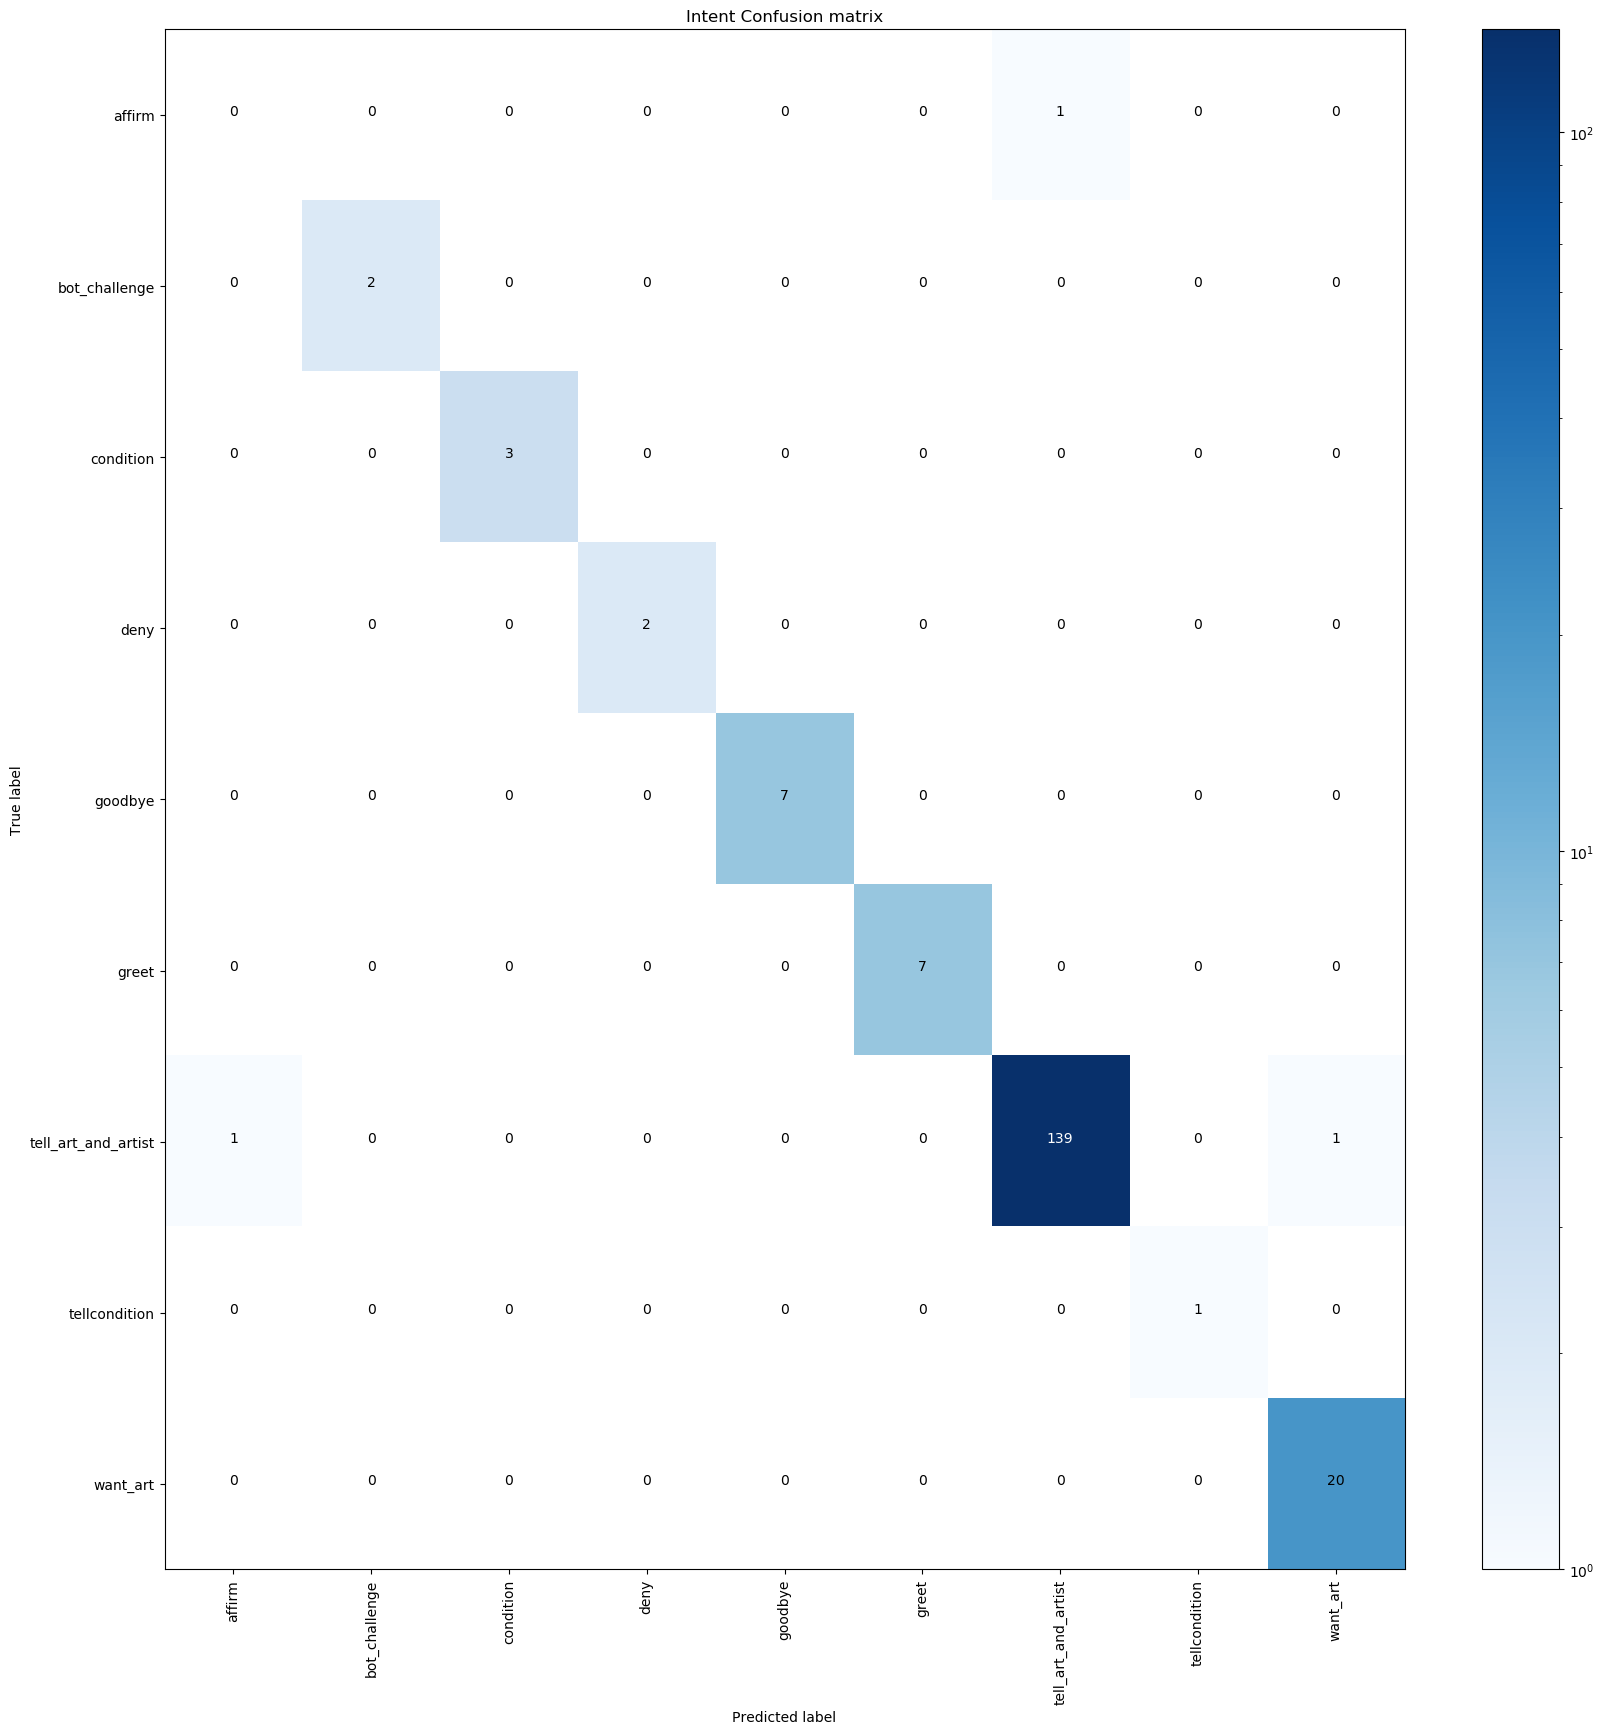
\includegraphics[width=1\linewidth]{figures/confmat.png}}
	\caption{Konfusionsmatrix des Klassifikationsergebnis von Rasa NLU.}
	\label{confnlu}
\end{figure}

\newpage

\section{Klassifikationsergebnis von Rasa Core (Fabio Aubele)}\label{anhang:core}
Dieser Anhang stellt das Klassifikationsergebnis von Rasa Core dar. Der Aufbau ist dabei derselbe wie bei Rasa NLU (Anhang \ref{anhang:nlu}). Jedoch sind die Labels auf den Achsen hierbei die entsprechenden Antworten des Chatbots, welche von dem neuronalen Netz bestimmt wurde. Am meisten tritt dabei 'action\_listen' auf, da diese Aktion immer ausgelöst wird, wenn der Chatbot eine neue Eingabe erwartet. Um alles vollständig lesen zu können, muss das Dokument eventuell etwas vergrößert werden, wenn es in digitaler Form vorliegt.
\begin{figure}[htbp]
	\centerline{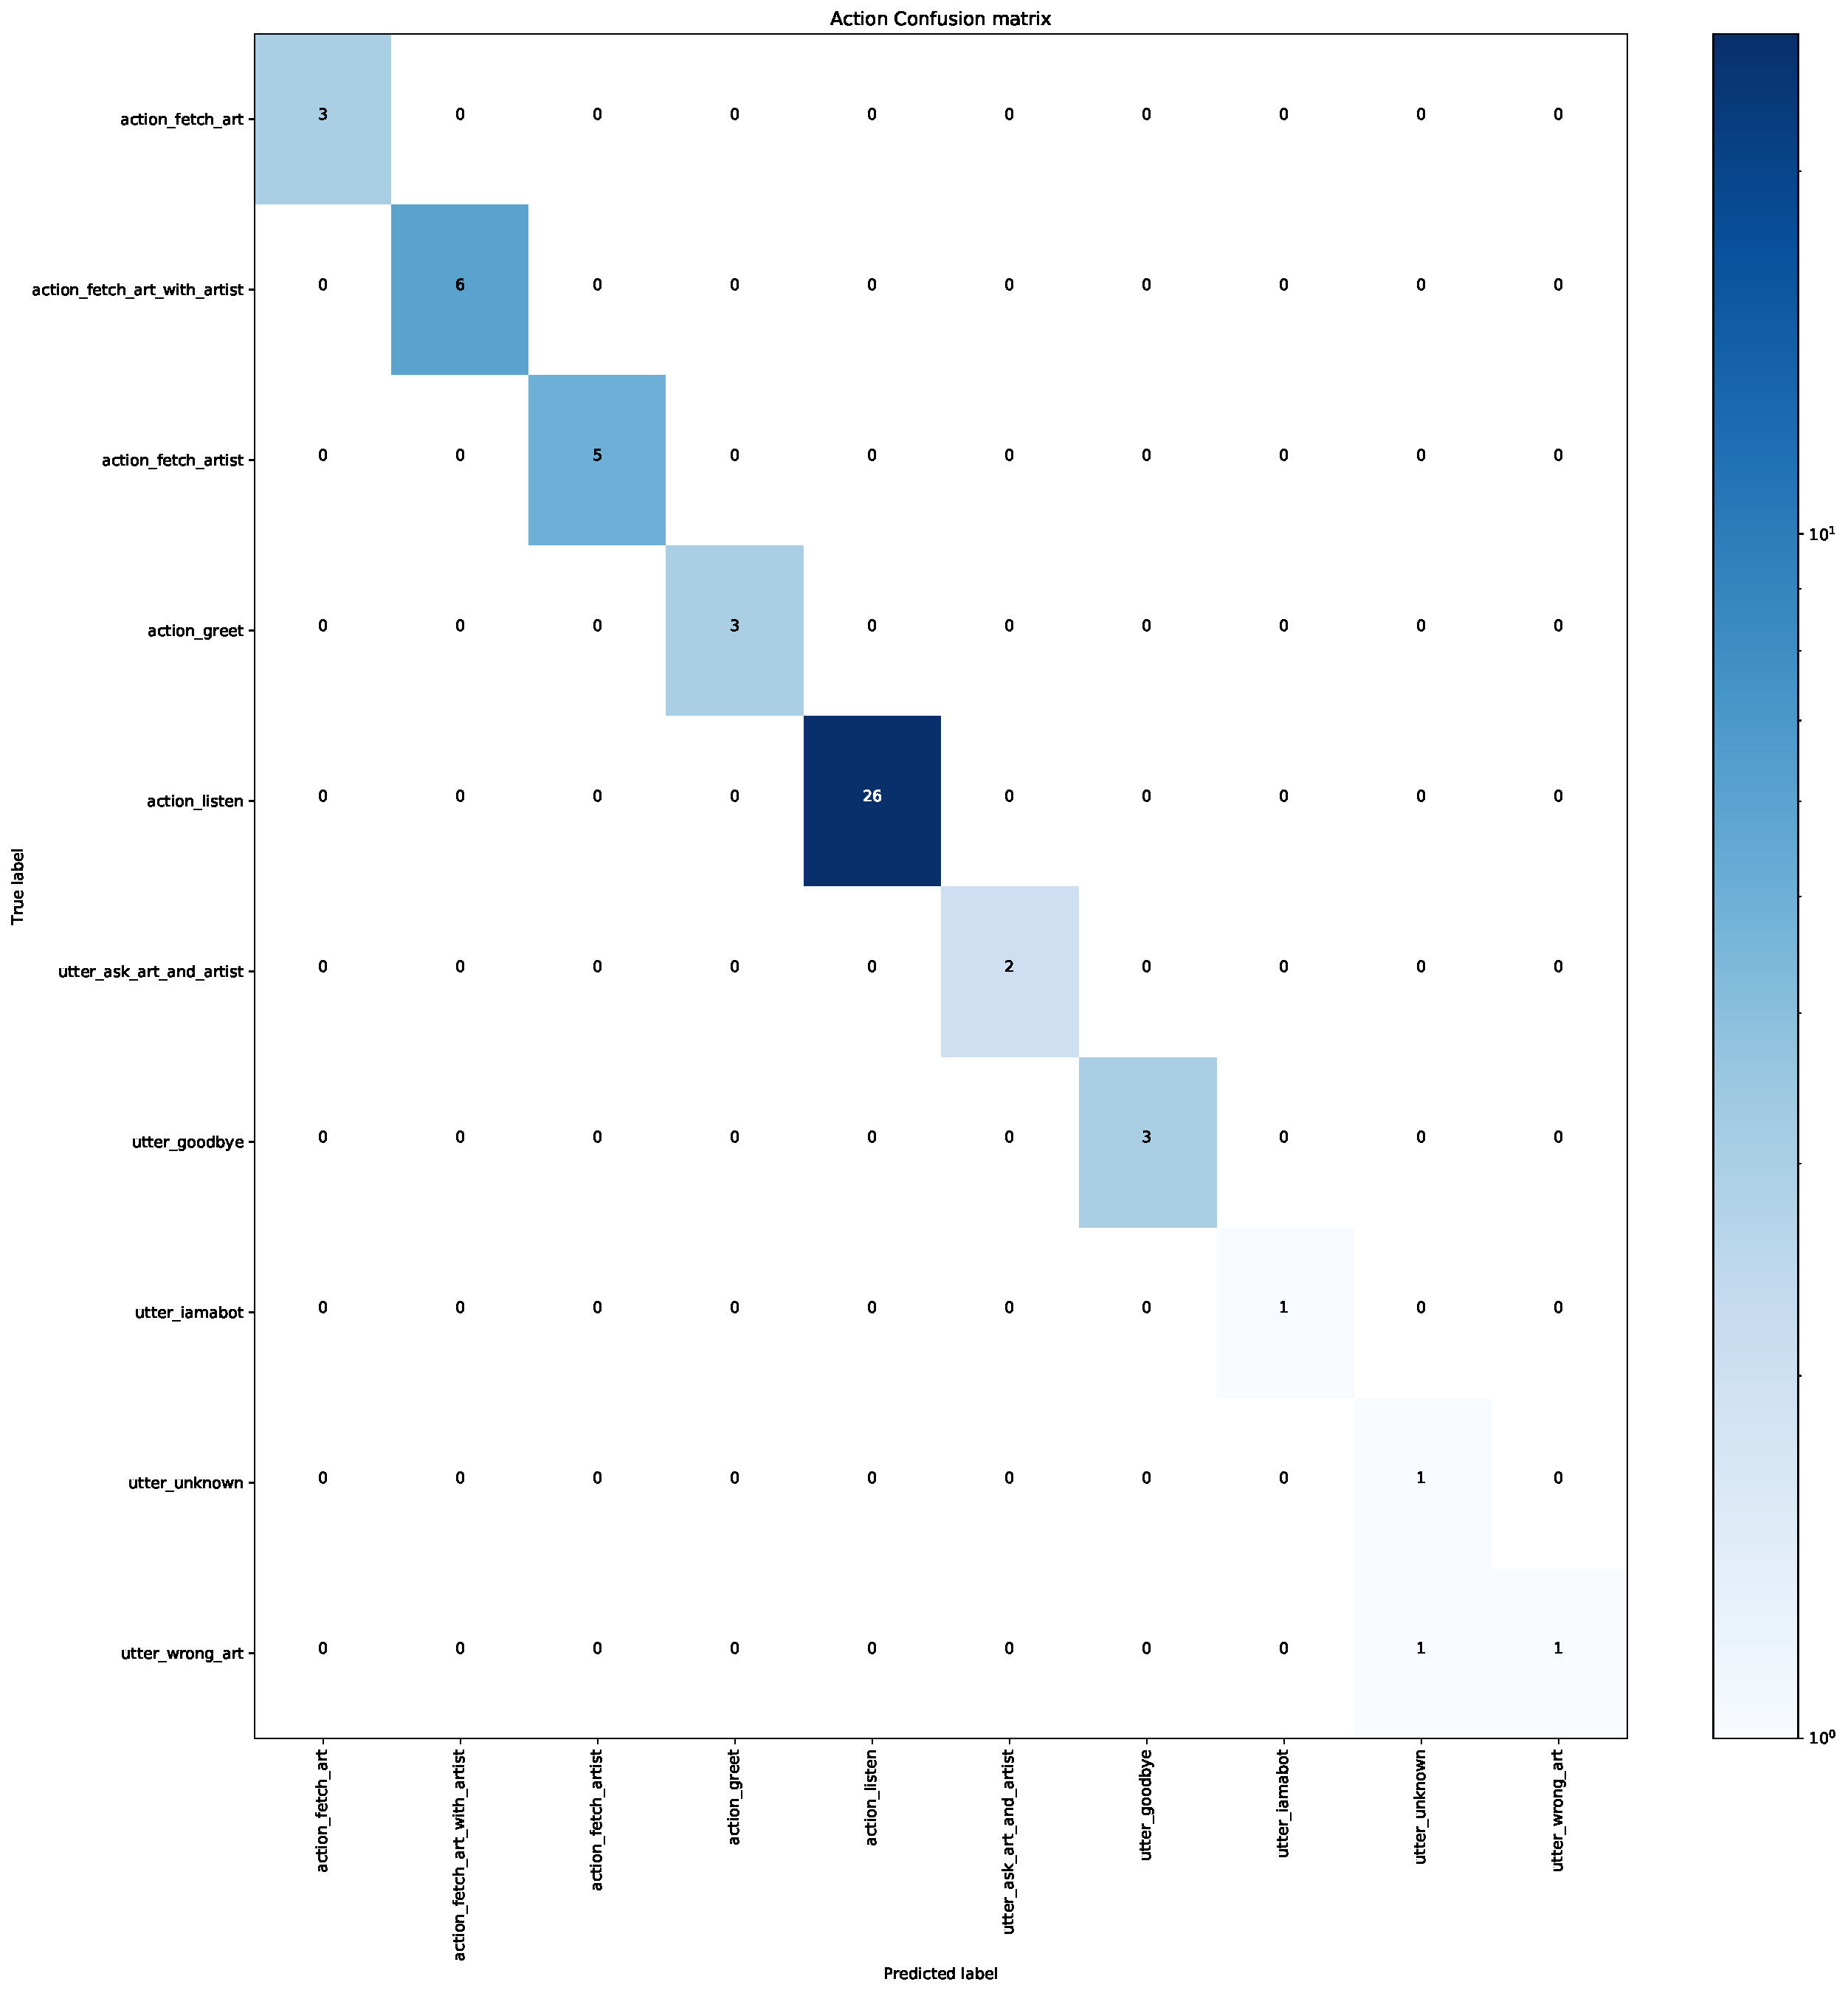
\includegraphics[width=1\linewidth]{figures/story_confmat.pdf}}
	\caption{Konfusionsmatrix des Klassifikationsergebnis von Rasa Core.}
	\label{confcore}
\end{figure}
	\end{appendices}
	
\end{document}